\chapter{Interrupts}
In dit hoofdstuk worden interrupts en het interruptmechanisme van de ATmega32
behandeld.

\section{Polling}
De ATmega32 kan met behulp van een wachtlus reageren op signalen van
externe bronnen. De externe bronnen kunnen zo aan de processor aangeven
dat er bijvoorbeeld data beschikbaar is en dat afhandeling is gewenst.
Dat werkt als volgt. De ATmega32 leest een byte in van een van de
I/O-poorten. Vervolgens wordt de bit die getest moet worden met behulp
van een bitmasker gefilterd. Is de geteste bit niet actief, dan wordt
opnieuw een byte ingelezen en begint het testen opnieuw. Is de geteste
bit wel actief, dan wordt de wachtlus verlaten en wordt de rest van het
programma uitgevoerd. 
Deze methode wordt \textsl{polling} genoemd. In het vakgebied van de
Operating Systems wordt dit \textsl{busy waiting} genoemd.

In listing~\ref{cod:intpolling} is een voorbeeld van zo'n wachtlus te zien.
Eerst wordt de status van de pinnen van Port A ingelezen door middel van
een \lstinline|in|-instructie. De \lstinline|andi|-instructie zorgt ervoor
dat de minst significante bit wordt gefilterd; de overige bits worden op~0
gezet. De \lstinline|andi|-instructie past ook de Z-vlag aan. Als blijkt
dat de minst significante bit een~0 is dan wordt de Z-vlag op~1 gezet,
anders wordt de Z-vlag op~0 gezet (merk op dat de overige bits op~0 gezet
zijn). Als blijkt dat de minst significante bit een~0 is, dan zorgt de
\lstinline|breq|-instructie ervoor dat weer naar het begin van de wachtlus
wordt gesprongen. Is de minst significante bit een~1, dan wordt de lus
verlaten en wordt de eerstvolgende instructie uitgevoerd. 

\begin{lstlisting}[language=AVRassembler,caption=Polling.,label=cod:intpolling]
loop:	in   r16,PINA   ; read in pins Port A
		andi r16,0x01   ; filter LSB, Z-flag = 1 if bit = 0
		breq loop       ; again if bit is 0
\end{lstlisting}

Deze manier van detectie werkt eenvoudig en snel. Het programma (de wachtlus)
is eenvoudig en er zijn slechts enkele klokpulsen nodig om de status van een
extern signaal te bepalen. Het nadeel is natuurlijk dat de processor niets
anders kan doen.


\section{Interrupts}
Slimmer is om de hardware aan de processor door te laten geven dat de status
van een signaal is veranderd, zodat de processor direct actie kan ondernemen.
Het lopende programma wordt dan \textsl{geïnterrumpeerd} (onderbroken).
Dit wordt een \textsl{interrupt} genoemd. Een aanvraag voor een onderbreking
(het signaal) wordt een \textsl{interrupt request} (IRQ) genoemd.

Nadat een interrupt request door de processor is herkend, wordt het lopende
programma onderbroken (de huidige instructie wordt afgemaakt) en wordt een
\textsl{interrupt service routine} (ISR) uitgevoerd. De ISR handelt dan de
interrupt verder af. Daarna gaat de processor verder waar het gebleven was.

We beelden dit uit in figuur~\ref{fig:intsimpleinterruptdispatch}. Hierin
stelt \textsf{H} de uitvoer van het lopende programma voor. Op een gegeven
moment wordt er een interrupt geregistreerd door de processor. Het lopende
programma wordt verlaten en de processor gaat de ISR uitvoeren. Aan het einde
van de ISR wordt teruggekeerd naar het lopende programma \textsf{H}.

\begin{figure}[!ht]
\centering
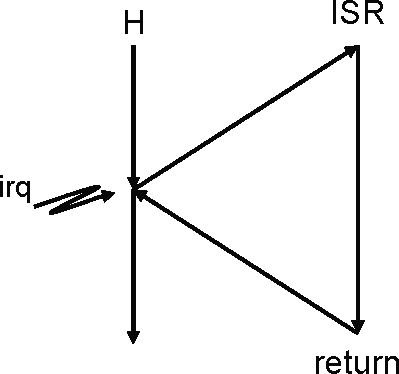
\includegraphics[scale=\figscale]{images/intsimpleinterruptdispatch}
\caption{Eenvoudige voorstelling van een interruptafhandeling.}
\label{fig:intsimpleinterruptdispatch}
\end{figure}

ISR's lijken veel op gewone subroutines, maar er zijn verschillen:

\begin{itemize}
\item Een ISR wordt gestart door een interrupt, niet door een
instructie\footnote{Er zijn processoren die instructies hebben die
software-interrupts genereren, zoals de Intel x86-familie.}.

\item Direct nadat de interrupt is herkend, wordt de Global Interrupt Enable
vlag (de I-vlag) in het Status Register op 0 gezet. Dit zorgt ervoor dat de
ISR niet kan worden onderbroken door een (nieuwe) interruptaanvraag.

\item Voor terugkeer moet de instructie \lstinline|reti| (Return From
Interrupt) gebruikt worden. Deze instructie zet de Global Interrupt Enable
vlag weer aan.
\end{itemize}

Interrupts en subroutines hebben wel \'e\'en overeenkomst: in beide gevallen
wordt de program counter (PC) op de stack gezet. Dit wordt uitgebeeld in
figuur~\ref{fig:intinterruptdispatchwithstackandiflag}. Omdat het
terugkeeradres op de stack wordt gezet, moet de stack pointer (SP) worden
ge\"initialiseerd v\'o\'ordat de interrupts mogen worden afgehandeld. Dat
betekent dat direct na het starten van het lopende programma, bijvoorbeeld
na een reset, de interrupts nog niet mogen worden afgehandeld omdat de
stack pointer nog niet is ge\"initialiseerd.

\begin{figure}[!ht]
\centering
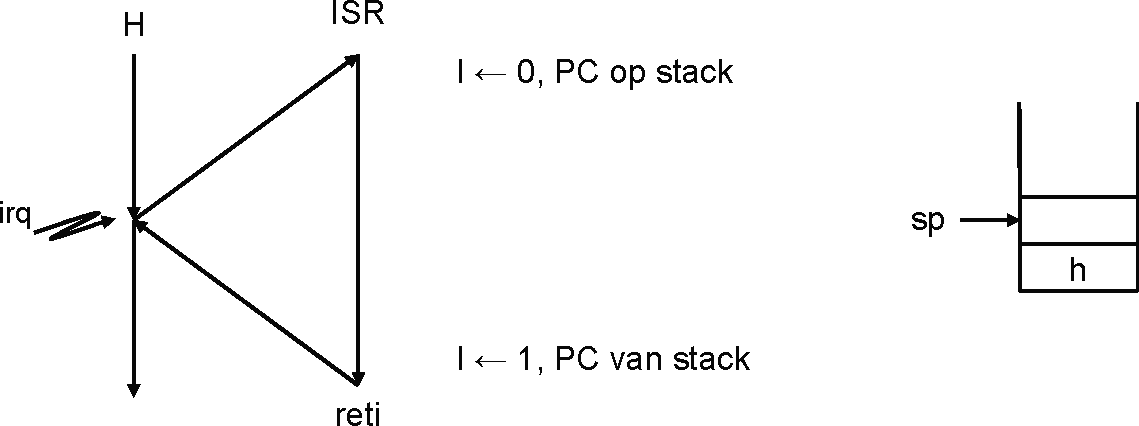
\includegraphics[scale=\figscale]{images/intinterruptdispatchwithstackandiflag}
\caption{Interruptafhandeling: de program counter wordt op de stack gezet.}
\label{fig:intinterruptdispatchwithstackandiflag}
\end{figure}

Twee instructies be\"invloeden direct de I-flag:

\qquad \lstinline|sei| - set Global Interrupt Enable flag, interrupts worden
afgehandeld.

\qquad\lstinline|cli| - clear Global Interrupt Enable flag, interrupts worden
geblokkeerd.

De I-vlag is gepositioneerd op bit 7 van het Status Register (SREG). Zie
figuur~\ref{fig:intsregregisterlayout}.

%%%% SREG
\begin{figure}[!ht]
\renewcommand\arraystretch{1.4}
%\footnotesize
\scriptsize
\centering
\begin{tabu} to 0.9\textwidth {X[,c,]X[,c,]X[,c,]X[,c,]X[,c,]X[,c,]X[,c,]X[,c,]}
7 & 6 & 5 & 4 & 3 & 2 & 1 & 0 \\
\hline
\multicolumn{1}{|c}{I} & \multicolumn{1}{|c}{T} & \multicolumn{1}{|c}{H} & \multicolumn{1}{|c}{S} & \multicolumn{1}{|c}{V} & \multicolumn{1}{|c}{N} & \multicolumn{1}{|c}{Z} & \multicolumn{1}{|c|}{C} \\ \hline
R/W & R/W & R/W & R/W & R/W & R/W & R/W & R/W \\
0 & 0 & 0 & 0 & 0 & 0 & 0 & 0 \\
\end{tabu}
\caption{Het Status Register SREG.}
\label{fig:intsregregisterlayout}
\end{figure}
%%%% SREG

Pas na het initialiseren van de stack pointer mag de instructie
\lstinline|sei| gegeven worden.


\section{Interruptbronnen}
De ATmega32 kent veel interruptbronnen. Zo kan de ATmega32 reageren op
drie externe interrupts: INT0, INT1 en INT2. Verder kan de analoog-digitaal
converter (ADC) een interrupt geven als de conversie klaar is. De seri\"ele
interface (USART) kent naast een interrupt wanneer een karakter is ontvangen
ook een interrupt voor wanneer een karakter is verzonden. De nog te bespreken
timer/counters (zie hoofdstuk~\ref{cha:timercounters}) kunnen een interrupt
afgeven wanneer een timer/counter ``over de kop'' gaat, dus wanneer een
timer/counter van de hoogste stand naar de laagste stand gaat. Verder zijn
er nog interrupts mogelijk van de EEPROM, de TWI- en de SPI-interface.

Al deze interruptbronnen hebben een eigen interrupt-enable-bit. Om een
interrupt van een bron ook daadwerkelijk te laten plaatsvinden, moet deze
bit geactiveerd zijn (logisch~1) \'en de I-vlag moet logisch 1 zijn.

De ATmega32 heeft geen \textsl{software interrupts}. Dat zijn
software-instructies die interrupts genereren. Deze zijn wel na te bootsen
met INT0, INT1 en INT2.


\section{De Interrupt Vector Table}
We hebben nu besproken hoe het verwerken van een interrupt wordt uitgevoerd.
Maar nu rijst de vraag: waar moet de ISR beginnen? We zouden hiervoor een
vast adres in de Flash-ROM kunnen kiezen, bijvoorbeeld adres 0x1000.
Vervolgens reserveren we 512 bytes voor de ISR. De volgende ISR begint dan
op adres 0x1200. Hoewel dit natuurlijk te realiseren is, kleven hier wel
wat nadelen aan. Ten eerste moet de ISR altijd op adres 0x1000 beginnen.
Ten tweede kan de ISR niet groter zijn dan 512 bytes. Als de ISR korter is
dan 512 bytes, dan gebruiken we een gedeelte van de Flash-ROM niet (bedenk
dat de volgende ISR op adres 0x1200 begint). Ten derde moet de Flash-ROM
minimaal 4608 (= 0x1200) bytes groot zijn. We zien nu dat een vast adres
en een vaste lengte voor een ISR niet flexibel is.

We kunnen deze drie problemen oplossen door gebruik te maken van een
\textsl{Interrupt Vector Table}. Dit werkt als volgt. Aan elke interrupt is
een zogenoemde \textsl{Interrupt Vector} gekoppeld. Dit is een vast adres
in de Flash-ROM waar naartoe gesprongen wordt als een interrupt is herkend.
Elke vector is twee words (vier bytes) groot. Na het herkennen van de
interrupt wordt de PC dus geladen met het adres van de Interrupt Vector die
bij de interrupt hoort.
Aangezien elke Interrupt Vector slechts twee words groot is, zal op die
plek een spronginstructie naar de eigenlijke ISR geplaatst worden. Het
uitvoeren gebeurt dus in twee stappen: eerst naar de Interrupt Vector
springen en van daaruit naar de eigenlijk ISR. Het gebruik van de
Interrupt Vector Table is weergegeven in
figuur~\ref{fig:intinterruptdispatchwithvectortable}.

\begin{figure}[!ht]
\centering
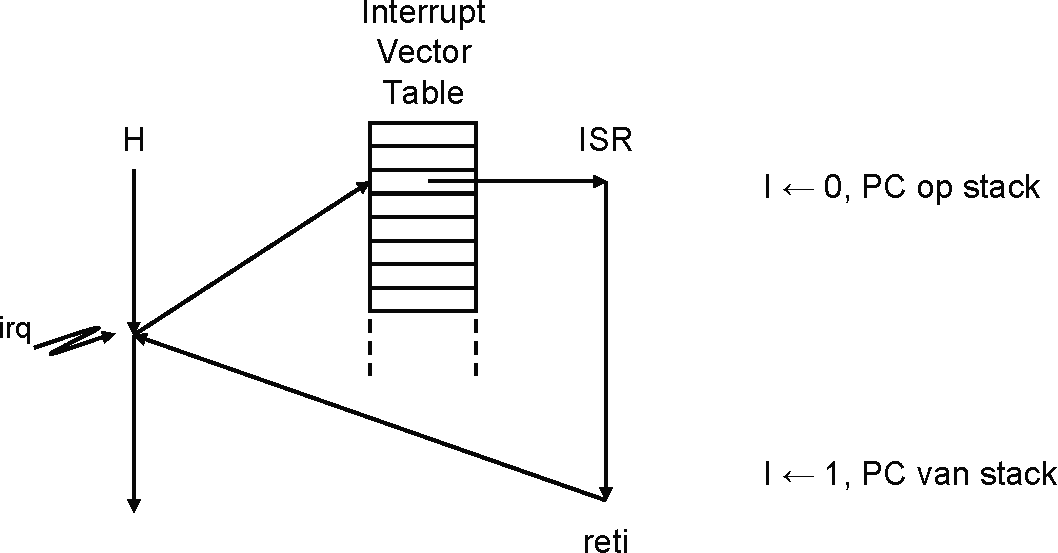
\includegraphics[scale=\figscale]{images/intinterruptdispatchwithvectortable}
\caption{Interruptafhandeling: gebruik van de Interrupt Vector Table.}
\label{fig:intinterruptdispatchwithvectortable}
\end{figure}

De Interrupt Vector Table ligt aan het begin van de Flash-ROM, van adres
0x000 t/m 0x029. Dat betekent dat de eerste vrije plaats 0x02a is. Vanaf
hier kan het gebruikersprogramma geplaatst worden. Na een reset is de PC
geladen met 0x000, dus wordt de instructieverwerking begonnen bij de eerste
vector. Deze is dan ook gereserveerd voor de Reset Vector. Op de Reset Vector
wordt dan een spronginstructie naar adres 0x02a geplaatst.

Natuurlijk heeft het gebruik van de Interrupt Vector Table een keerzijde.
Zo zijn er extra geheugenplaatsen nodig voor het opslaan van de vectoren.
De executietijd van de interrupt (Engels: interrupt latency) wordt met
drie klokpulsen verhoogd omdat er een sponginstructie moet worden uitgevoerd.

Een overzicht van de Interrupt Vector Table is te vinden in
tabel~\ref{tab:intinterruptvectortable}. Op adres 0x000 is de Reset Vector
geplaatst. Daarna volgt op adres 0x002 de vector voor de eerste externe
interrupt, dan voor de tweede externe interrupt, enzovoorts.

\begin{table}[!ht]
\centering
\caption{Interruptvectortabel voor de ATmega32.}
\label{tab:intinterruptvectortable}
\setlength{\tabcolsep}{8pt}
\begin{tabu}{ccll}
\toprule
vector \# & ROM-adres & Bron          & Omschrijving \\ \midrule
 1        & 0x000     & RESET         & Reset vector \\
 2        & 0x002     & INT0          & External Interrupt request 0 \\
 3        & 0x004     & INT1          & External Interrupt request 1 \\
 4        & 0x006     & INT2          & External Interrupt request 2 \\
 5        & 0x008     & TIMER2\_COMP  & Timer/Counter2 Compare Match \\
 6        & 0x00A     & TIMER2\_OVF   & Timer/Counter2 Overflow \\
 7        & 0x00C     & TIMER1\_CAPT  & Timer/Counter1 Capture Event \\
 8        & 0x00E     & TIMER1\_COMPA & Timer/Counter1 Compare Match A \\
 9        & 0x010     & TIMER1\_COMPB & Timer/Counter1 Compare Match B \\
10        & 0x012     & TIMER1\_OVF   & Timer/Counter1 Overflow \\
11        & 0x014     & TIMER0\_COMP  & Timer/Counter0 Compare Match \\
12        & 0x016     & TIMER0\_OVF   & Timer/Counter0 Overflow \\
13        & 0x018     & SPI, STC      & Serial Transfer Complete \\
14        & 0x01A     & USART, RXC    & USART, Rx Complete \\
15        & 0x01C     & USART, UDRE   & USART Data Register Empty \\
16        & 0x01E     & USART, TXC    & USART, Tx Complete \\
17        & 0x020     & ADC           & ADC Conversion Complete \\
18        & 0x022     & EE\_RDY       & EEPROM Ready \\
19        & 0x024     & ANA\_COMP     & Analog Comparator \\
20        & 0x026     & TWI           & Two-wire Serial Interface \\
21        & 0x028     & SPM\_RDY      & Store Program Memory Ready \\
\bottomrule
\end{tabu}
Noot: het ROM-adres is in words.
\end{table}


\section{Interruptpriotiteit}
Als twee interrupt tegelijk binnenkomen, wordt de interrupt met de laagste
Interrupt Vector als eerste uitgevoerd. Er zijn dus prioriteiten aan de
interrupts gekoppeld. De interrupt die op dat moment niet wordt uitgevoerd,
moet wachten totdat de uitgevoerde interrupt afgehandeld is. Komt er echter
in de tussentijd een interrupt binnen met een lagere Interrupt Vector
dan wordt die weer als eerste uitgevoerd.


\section{Stappen in de interruptverwerking}
Als een interruptsignaal bij de processor binnenkomt, worden de volgende
stappen genomen:
\begin{enumerate}
\item De processor maakt de instructie af die op dat moment wordt uitgevoerd.
      Dit is een instructie in het lopende programma.
\item De processor slaat het adres van de volgende instructie op de stack op.
      Dit adres staat in de program counter. De Global Interrupt Enable vlag
      wordt op 0 gezet.
\item De processor springt naar de interrupt vector. Dit is een vaste
      geheugenlocatie in de Flash-ROM.
\item Vanuit de interrupt vector wordt gesprongen naar het adres van de
      daadwerkelijke ISR.
\item Bij terugkeer uit de ISR wordt de program counter geladen met het adres
      dat op de stack gezet was. De Global Interrupt Enable vlag wordt op 1
      gezet.
\item De processor vervolgt het uitvoeren van het programma. Er wordt altijd
      \'e\'en instructie uitgevoerd voordat een eventuele nieuwe interrupt
      wordt verwerkt.
\end{enumerate}


\section{Interruptresponstijd}
De responstijd voor alle ingeschakelde interrupts van de ATmega32 is minimaal
vier klokcycli. Tijdens deze vier klokcycli wordt de program counter op de
stack geplaatst (twee bytes) en wordt de program counter geladen met het
vectoradres van de interrupt. Na vier klokcycli wordt gesprongen naar het
vectoradres van de interrupt die wordt verwerkt. De instructie op de vector
is normaal gesproken een sprong naar de interruptroutine en deze sprong duurt
drie klokcycli voor een \lstinline|jmp|-instructie en twee klokcycli voor een
\lstinline|rjmp|-instructie.

Als een interrupt optreedt tijdens de uitvoering van een instructie met
meerdere klokcycli dan wordt deze instructie afgemaakt voordat de interrupt
wordt verwerkt. Staat de ATmega32 in slaapstand dan wordt de responstijd met
vier klokcycli verhoogd. Deze verhoging komt bovenop de opstarttijd van de
geselecteerde slaapmodus.

Een terugkeer (return) uit een interruptroutine duurt vier klokcycli. Tijdens
deze vier klokcycli wordt de program counter van de stack gehaald (twee bytes)
en wordt de stack pointer met twee verhoogd. Tevens wordt de I-bit in het
statusregister op 1 gezet.

\section{Context switch}
Een interrupt kan op elk willekeurig moment plaatsvinden. We noemen zulke
interrupts \textsl{asynchroon}. Asynchroon houdt in dat het moment van
de interrupt niet (helemaal) te voorspellen is\footnote{Interrupts van
bijvoorbeeld de timer/counters zijn natuurlijk wel uit te rekenen.}. Stel
dat het lopende programma een complexe berekening aan het uitvoeren is.
De berekening zorgt ervoor dat de vlaggen en de registers worden aangepast.
Als nu een interrupt binnenkomt en de ISR wordt gestart dan is er een
grote kans dat in de ISR ook registers en de vlaggen worden aangepast.
Bij terugkeer naar het lopende programma moeten dan de originele waarden
van de registers en de vlaggen weer beschikbaar zijn om de berekening
correct te laten verlopen, d.w.z.\@ dat de \textsl{context} weer hersteld
moet worden. Het is daarom belangrijk om in de ISR de gebruikte registers
en de vlaggen op te slaan. Dat kan door gebruik te maken van de stack. 

In listing~\ref{cod:intcontextswich} is te zien hoe de vlaggen op de stack
geplaatst worden. De vlaggen zijn op te vragen via I/O-register
\lstinline|SREG|. Nu kan de inhoud van een I/O-register niet direct op de
stack geplaatst worden. Dit moet via een register. Dat betekent dat de inhoud
van dat register eerst op de stack geplaatst moet worden. Daarna worden de
vlaggen ingelezen in het register en op de stack gezet.

\begin{figure}[!ht]
\begin{lstlisting}[language=AVRassembler,caption=Opslaan van de registers en vlaggen.,label=cod:intcontextswich]
ISR:	push r16		; push R16
		in   r16,SREG	; SREG in I/O memory ...
		push r16		; ... so push flags via R16
		
		; rest of the ISR code

		pop  r16		; pop flags via R16
		out  SREG,r16
		pop  r16		; pop R16
		reti			; return
\end{lstlisting}
\end{figure}

Aan het einde van de ISR moeten de registers en de vlaggen weer van de stack
gehaald worden. Let daarbij op de volgorde van de registers.


\section{Externe interrupts}
De ATmega32 kent drie externe interrupts genaamd INT0, INT1 en INT2. Deze
interrupts zijn fysiek verbonden met Port D, bit 2 (PD2, INT0), Port D, bit
3 (PD3, INT1) en Port B, bit 2 (PB2, INT2). INT0 en INT1 kunnen zowel op een
laag niveau als op flanken reageren. INT2 kan alleen op flanken reageren.
Zoals te
zien in tabel~\ref{tab:intinterruptvectortable} worden de vectoradressen
0x002, 0x004 en 0x006 gebruikt voor respectievelijk INT0, INT1, en INT2. We
merken op dat INT0 dus een hogere prioriteit heeft dan INT1 en INT2.

Om een externe interrupt te herkennen, moeten de bijbehorende pinnen als
ingang gedefinieerd worden. Maar er moet opgemerkt worden dat interrupts
ook worden herkend als de bijbehorende pin als uitgang gedefinieerd is. Op
deze manier is het mogelijk om vanuit de software een interrupt te genereren. 

Het General Interrupt Control Register (GICR) heeft drie bits waarmee de INT’s
kunnen worden geactiveerd. Een logische 1 in de betreffende bit activeert de
INT. Merk op dat de I-vlag in het Status Reister 1 moet zijn om interrupt ook
daadwerkelijk te laten plaatsvinden. De indeling van het GICR is te vinden in
figuur~\ref{fig:intgicr}. Alleen de bits 5, 6 en~7 zijn van belang. 

%%%% GICR
\begin{figure}[!ht]
\renewcommand\arraystretch{1.4}
%\footnotesize
\scriptsize
\centering
\begin{tabu} to 0.9\textwidth {X[,c,]X[,c,]X[,c,]X[,c,]X[,c,]X[,c,]X[,c,]X[,c,]}
7 & 6 & 5 & 4 & 3 & 2 & 1 & 0 \\
\hline
\multicolumn{1}{|c}{INT1} & \multicolumn{1}{|c}{INT0} & \multicolumn{1}{|c}{INT2} & \multicolumn{1}{|c}{\cellcolor{lightgrey} $-$} & \multicolumn{1}{|c}{\cellcolor{lightgrey} $-$} & \multicolumn{1}{|c}{\cellcolor{lightgrey} $-$} & \multicolumn{1}{|c}{\cellcolor{lightgrey} IVSEL} & \multicolumn{1}{|c|}{\cellcolor{lightgrey} IVCE} \\ \hline
R/W & R/W & R/W & R & R & R & R/W & R/W \\
0 & 0 & 0 & 0 & 0 & 0 & 0 & 0 \\
\end{tabu}
\caption{Het GICR register.}
\label{fig:intgicr}
\end{figure}
%%%% GICR

In listing~\ref{cod:intenableint0} is te zien hoe INT0 geactiveerd wordt.
Merk op dat de betreffende bit in het Data Direction Register D (DDRD, bit 2)
op 0 moet staan om de pin als ingang te defini\"eren.

\begin{figure}[!ht]
\begin{lstlisting}[language=AVRassembler,caption=Het activeren van INT0.,label=cod:intenableint0]
    ldi r16,0b01000000  ; activate INT0 (pin PD2)
    out GICR,r16
\end{lstlisting}
\end{figure}

Een flankgevoelige interrupt (opgaande flank, neergaande flank of beide
flanken) wordt door de ATmega32 ``ingevangen''. Dit wordt bijgehouden in
het General Interrupt Flag Register (GIFR). Dat betekent dat als een
flankgevoelige interrupt wordt herkend, de bijbehorende bit in het
GIFR-register op 1 wordt gezet. Als de ISR wordt uitgevoerd, wordt de
bit door de hardware op 0 gezet. Zolang een interruptaanvraag niet
wordt uitgevoerd blijft de bit dus 1. In figuur~\ref{fig:intgifr} is
de indeling van het GIFR-register te zien. Merk op dat een niveaugevoelige
interrupt (INT0, INT1) de bijbehorende bits in het GIFR-register niet op
1 zet. Bij niveaugevoelige interrupts wordt direct de status van de pinnen
ingelezen.

%%%% GIFR
\begin{figure}[!ht]
\renewcommand\arraystretch{1.4}
%\footnotesize
\scriptsize
\centering
\begin{tabu} to 0.9\textwidth {X[,c,]X[,c,]X[,c,]X[,c,]X[,c,]X[,c,]X[,c,]X[,c,]}
7 & 6 & 5 & 4 & 3 & 2 & 1 & 0 \\
\hline
\multicolumn{1}{|c}{INTF1} & \multicolumn{1}{|c}{INTF0} & \multicolumn{1}{|c}{INTF2} & \multicolumn{1}{|c}{\cellcolor{lightgrey} $-$} & \multicolumn{1}{|c}{\cellcolor{lightgrey} $-$} & \multicolumn{1}{|c}{\cellcolor{lightgrey} $-$} & \multicolumn{1}{|c}{\cellcolor{lightgrey} $-$} & \multicolumn{1}{|c|}{\cellcolor{lightgrey} $-$} \\ \hline
R/W & R/W & R/W & R & R & R & R & R \\
0 & 0 & 0 & 0 & 0 & 0 & 0 & 0 \\
\end{tabu}
\caption{Het GIFR register.}
\label{fig:intgifr}
\end{figure}
%%%% GIFR

Merk op dat een bit in het GIFR-register door software op 0 kan worden gezet
door er een 1 naar toe te schrijven. Dit principe geldt voor alle interrupts
die de ATmega32 kent.

\subsubsection*{Triggermogelijkheden van INT0 en INT1}
Zowel INT0 als INT1 kunnen op meerdere mogelijkheden geactiveerd worden.
Ze kunnen reageren op een laag niveau, op een opgaande flank, op een
neergaande flank of op beide flanken. Ze kunnen niet reageren op een
hoog niveau. De mogelijkheden worden aangegeven met de ISC-bits in het
MCU Control Register (MCUCR). De indeling van dit register is te zien
in figuur~\ref{fig:intmcucr}. 

%%%% MCUCR
\begin{figure}[!ht]
\renewcommand\arraystretch{1.4}
%\footnotesize
\scriptsize
\centering
\begin{tabu} to 0.9\textwidth {X[,c,]X[,c,]X[,c,]X[,c,]X[,c,]X[,c,]X[,c,]X[,c,]}
7 & 6 & 5 & 4 & 3 & 2 & 1 & 0 \\
\hline
\multicolumn{1}{|c}{\cellcolor{lightgrey} SE} & \multicolumn{1}{|c}{\cellcolor{lightgrey} SM2} & \multicolumn{1}{|c}{\cellcolor{lightgrey} SM1} & \multicolumn{1}{|c}{\cellcolor{lightgrey} SM0} & \multicolumn{1}{|c}{ISC11} & \multicolumn{1}{|c}{ISC10} & \multicolumn{1}{|c}{ISC01} & \multicolumn{1}{|c|}{ISC00} \\ \hline
R/W & R/W & R/W & R/W & R/W & R/W & R/W & R/W \\
0 & 0 & 0 & 0 & 0 & 0 & 0 & 0 \\
\end{tabu}
\caption{Het MCUCR register.}
\label{fig:intmcucr}
\end{figure}
%%%% MCUCR

\textbf{Bit 3, 2 – ISC11, ISC10: Interrupt Sense Control 1 bit 1 en bit 0} \\
De ISC11- en ISC10-bits defini\"eren de wijze waarop INT1 een interrupt
genereert. De INT1-pin (PD3) wordt bemonsterd voordat de flank wordt
gedetecteerd. Als flankgevoelige triggering is geselecteerd, worden pulsen
groter dan \'e\'en klokcyclus herkend. Als een puls korter is dan \'e\'en
klokcyclus dan is er geen garantie dat de puls (en dus de flank) wordt
herkend. Als triggering van een laag niveau wordt gebruikt, dan moet het
lage niveau aangehouden worden totdat de huidige instructie uitgevoerd is.
De langstdurende instructie is een \lstinline|call|-instructie. Deze
instructie duurt op een ATmega32 vier klokcycli. Dat betekent dat het
lage niveau op de INT1-pin dus minimaal vier klokcycli moet duren. De
interrupt wordt (steeds) herkend zolang het lage niveau aangehouden wordt.
In figuur~\ref{tab:inttriggerint1} is te zien hoe een bepaalde triggering
ingesteld moet worden.

\begin{table}[!ht]
\centering
\caption{Triggermogelijkheden van INT1.}
\label{tab:inttriggerint1}
\setlength{\tabcolsep}{8pt}
\begin{tabular}  {>{\centering\arraybackslash}m{1cm}>{\centering\arraybackslash}m{1cm}>{\centering\arraybackslash}m{2cm}m{7cm}}
\toprule
ISC11 & ISC10 & & Omschrijving \\ \midrule
  0   &   0   & 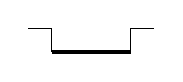
\begin{tikzpicture}\draw (0,0.3) -- (0.3,0.3) -- (0.3,0);\draw [ultra thick] (0.3,0.0) -- (1.3,0);\draw (1.3,0) -- (1.3,0.3) -- (1.6,0.3);\end{tikzpicture} & Een laag niveau op de INT1-ingang genereert een interrupt. \\ \midrule
  0   &   1   & 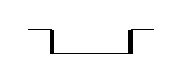
\begin{tikzpicture}\draw (0,0.3) -- (0.3,0.3);\draw [ultra thick] (0.3,0.3) -- (0.3,0.0);\draw (0.3,0) -- (1.3,0);\draw [ultra thick] (1.3,0) -- (1.3,0.3);\draw (1.3,0.3) -- (1.6,0.3);\end{tikzpicture} & Een opgaande en neergaande flank op de INT1-ingang genereert een interrupt. \\ \midrule
  1   &   0   & \begin{tikzpicture}\draw (0,0.3) -- (0.3,0.3);\draw [ultra thick] (0.3,0.3) -- (0.3,0.0);\draw (0.3,0) -- (1.3,0);\draw (1.3,0) -- (1.3,0.3);\draw (1.3,0.3) -- (1.6,0.3);\end{tikzpicture} & Een neergaande flank op de INT1-ingang genereert een interrupt. \\ \midrule
  1   &   1   & \begin{tikzpicture}\draw (0,0.3) -- (0.3,0.3);\draw (0.3,0.3) -- (0.3,0.0);\draw (0.3,0) -- (1.3,0);\draw [ultra thick] (1.3,0) -- (1.3,0.3);\draw (1.3,0.3) -- (1.6,0.3);\end{tikzpicture} & Een opgaande flank op de INT1-ingang genereert een interrupt. \\
\bottomrule
\end{tabular}
\end{table}

\newpage
In listing~\ref{cod:intenablerisingedgeint1} is te zien hoe INT1 wordt
ingesteld voor het herkennen van een opgaande flank om een interrupt te
genereren.

\begin{figure}[!ht]
\begin{lstlisting}[language=AVRassembler,caption=Instellen van de opgaande  flank voor INT11.,label=cod:intenablerisingedgeint1]
    ldi r16,0b00001100  ; activate rising edge INT1
    out MCUCR,r16
\end{lstlisting}
\end{figure}

\textbf{Bit 1, 0 – ISC01, ISC00: Interrupt Sense Control 0 bit 1 en bit 0} \\
De ISC01- en ISC00-bits defini\"eren de wijze waarop INT0 een interrupt
genereert. De werking is identiek aan die van de ISC-bits van INT1. Ook de
timing is identiek. Zie tabel~\ref{tab:inttriggerint0}.

\begin{table}[!ht]
\centering
\caption{Triggermogelijkheden van INT0.}
\label{tab:inttriggerint0}
\setlength{\tabcolsep}{8pt}
\begin{tabular}  {>{\centering\arraybackslash}m{1cm}>{\centering\arraybackslash}m{1cm}>{\centering\arraybackslash}m{2cm}m{7cm}}
\toprule
ISC01 & ISC00 & & Omschrijving \\ \midrule
  0   &   0   & 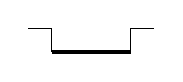
\begin{tikzpicture}\draw (0,0.3) -- (0.3,0.3) -- (0.3,0);\draw [ultra thick] (0.3,0.0) -- (1.3,0);\draw (1.3,0) -- (1.3,0.3) -- (1.6,0.3);\end{tikzpicture} & Een laag niveau op de INT0-ingang genereert een interrupt. \\ \midrule
  0   &   1   & 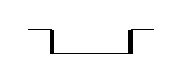
\begin{tikzpicture}\draw (0,0.3) -- (0.3,0.3);\draw [ultra thick] (0.3,0.3) -- (0.3,0.0);\draw (0.3,0) -- (1.3,0);\draw [ultra thick] (1.3,0) -- (1.3,0.3);\draw (1.3,0.3) -- (1.6,0.3);\end{tikzpicture} & Een opgaande en neergaande flank op de INT0-ingang genereert een interrupt. \\ \midrule
  1   &   0   & \begin{tikzpicture}\draw (0,0.3) -- (0.3,0.3);\draw [ultra thick] (0.3,0.3) -- (0.3,0.0);\draw (0.3,0) -- (1.3,0);\draw (1.3,0) -- (1.3,0.3);\draw (1.3,0.3) -- (1.6,0.3);\end{tikzpicture} & Een neergaande flank op de INT0-ingang genereert een interrupt. \\ \midrule
  1   &   1   & \begin{tikzpicture}\draw (0,0.3) -- (0.3,0.3);\draw (0.3,0.3) -- (0.3,0.0);\draw (0.3,0) -- (1.3,0);\draw [ultra thick] (1.3,0) -- (1.3,0.3);\draw (1.3,0.3) -- (1.6,0.3);\end{tikzpicture} & Een opgaande flank op de INT0-ingang genereert een interrupt. \\
\bottomrule
\end{tabular}
\end{table}

\subsubsection*{Triggermogelijkheden van INT2}
Externe interrupt INT2 kan alleen op de opgaande flank of op de neergaande
flank triggeren. Dit is in te stellen in het MCU Control and Status Register
(MCUCSR). De indeling van dit register is te zien in
figuur~\ref{fig:intmcucsr}. INT2 wordt \textsl{asynchroon} verwerkt.
Asynchroon betekent hier dat het interruptsignaal buiten de klok om wordt
``ingevangen''. De minimale pulsduur van INT2 is 50 ns, maar de puls wordt
dus niet bemonsterd op klokflanken van de systeemklok. De aanvraag wordt
wel verwerkt op de flanken van de systeemklok.

%%%% MCUCSR
\begin{figure}[!ht]
\renewcommand\arraystretch{1.4}
%\footnotesize
\scriptsize
\centering
\begin{tabu} to 0.9\textwidth {X[,c,]X[,c,]X[,c,]X[,c,]X[,c,]X[,c,]X[,c,]X[,c,]}
7 & 6 & 5 & 4 & 3 & 2 & 1 & 0 \\
\hline
\multicolumn{1}{|c}{\cellcolor{lightgrey} JTD} & \multicolumn{1}{|c}{ISC2} & \multicolumn{1}{|c}{\cellcolor{lightgrey} $-$} & \multicolumn{1}{|c}{\cellcolor{lightgrey} JTRF} & \multicolumn{1}{|c}{\cellcolor{lightgrey} WDRF} & \multicolumn{1}{|c}{\cellcolor{lightgrey} BORF} & \multicolumn{1}{|c}{\cellcolor{lightgrey} EXTRF} & \multicolumn{1}{|c|}{\cellcolor{lightgrey} PORF} \\ \hline
R/W & R/W & R & R/W & R/W & R/W & R/W & R/W \\
0 & 0 & 0 & 0 & 0 & 0 & 0 & 0 \\
\end{tabu}
\caption{Het MCUCSR register.}
\label{fig:intmcucsr}
\end{figure}
%%%% MCUCSR

\textbf{Bit 6 - ISC2: Interrupt Sense Control 2}\\
Bit ISC2 geeft aan op welke flank INT2 moet reageren. Een 0 geeft aan dat INT2
op een neergaande flank triggert, een 1 geeft aan dat INT2 op een opgaande
flank triggert.

Bij het wijzigen van de ISC2-bit kan een interrupt optreden. Daarom is het
nodig om INT2 eerst uit te schakelen door het uitschakelen van de INT2-bit
in het GICR-register. Vervolgens kan de ISC2-bit worden gewijzigd. Daarna
moet een eventuele interruptaanvraag worden gewist door een logische 1
naar de INTF2-bit in het GIFR-register te schrijven voordat de interrupt
opnieuw wordt ingeschakeld. In listing~\ref{cod:intexamplecodeint2} is te
zien hoe van flank kan worden gewisseld.

\begin{figure}[!ht]
\begin{lstlisting}[language=AVRassembler,caption=Omschakelen van INT2 van neergaande naar opgaande flank.,label=cod:intexamplecodeint2]
    ; Disable INT2, leave INT0/INT1 untouched
    in   r16,GICR
    andi r16,0b11011111
    out  GICR,r16
    
    ; Change falling edge to rising edge, don't touch other flags
    in   r16,MCUCSR
    ori  r16,0b01000000
    out  MCUCSR,r16
    
    ; Clear INTF2 flag
    ldi  r16,0x00100000
    out  GIFR,r16
    
    ; Enable INT2, leave INT0/INT1 untouched
    in   r16,GICR
    ori  r16,0b00100000
    out  GICR,r16
\end{lstlisting}
\end{figure}

In listing~\ref{cod:intexamplecodeint0} is een voorbeeld te zien van het
gebruik van INT0. Als taak heeft de ISR om de bits van Port B te
inverteren. We beginnen met het aangeven van de reset-vector (regel~5) en de
INT0-vector (regel~8). Daarna wordt de stack ge\"initialiseerd (regel~14
t/m~17). In regel~20 en~21 wordt Port B als uitgang ingesteld. In regel~24
en~25 wordt gekozen voor de opgaande flank van INT0. In regel~25 en~26
activeren we INT0. Daarna worden de interrupts vrij gegeven middels een
\lstinline|sei|-instructie (regel~32) en blijven we in een eeuwig durende lus
wachten (regel~35).

\begin{figure}[!p]
\begin{lstlisting}[language=AVRassembler,caption=Voorbeeldprogramma INT0 met opgaande flank en ISR.,label=cod:intexamplecodeint0]
.def temp = r16

.org 0x000
        ; reset vector
		rjmp reset
.org 0x002
        ; ISR vector for INT0
		rjmp int0_isr

.org 0x02a
        ; main program starts here
reset:
		; set up stack pointer
		ldi	 temp,low(RAMEND)
		out	 SPL,temp
		ldi	 temp,high(RAMEND)
		out	 SPH,temp
		
		; All pins Port B are outputs
		ldi  temp,0xff
		out  DDRB,temp

		; set up rising edge INT0
		ldi	 temp,0b00000011
		out	 MCUCR,temp

		; set up INT0
		ldi	 temp,0b01000000
		out	 GICR,temp

		; enable interrupts
		sei

		; forever....
loop: 	rjmp loop

int0_isr:
        ; save regs and flags
		push temp
		in   temp,SREG
		push temp

        ; Invert all Port B bits
        in   temp,PORTB
        com  temp
        out  PORTB,temp

		; restore regs and flags and return from interrupt
		pop	 temp
		out	 SREG,temp
		pop	 temp
 		reti
\end{lstlisting}
\end{figure}

In de ISR wordt de context (de processorstatus) op de stack gezet (regels~39
t/m~31). Daarna wordt Port B ingelezen, ge\"inverteerd en weer
teruggeschreven (regels~44 t/m~46). Vlak voor het terugkeren wordt de context
weer van de stack gehaald (regels~49 t/m~41). Daarna keren we weer terug naar
het lopende programma door middel van een \lstinline|reti|-instructie.

\section{Interrupts binnen interrupts}
Als een interrupt wordt afgehandeld, wordt de bijbehorende ISR gestart. Net
voordat ISR wordt gestart, wordt de Global Interrupt Enable vlag (I-vlag)
op~0 gezet. Dit zorgt ervoor dat nieuwe interruptaanvragen (nog) niet
afgehandeld worden. Deze aanvragen moeten wachten totdat de ISR klaar is.
Bij het terugkeren wordt de I-vlag weer op~1 gezet, zodat wachtende
interruptaanvragen kunnen worden afgehandeld.

Het is mogelijk om in een ISR de I-vlag weer op~1 te zetten zodat een
interruptaanvraag kan worden bediend. De ISR wordt dus onderbroken door
een interrupt en er wordt een (andere) ISR gestart. We spreken dan over
een interrupt binnen een interrupt.

Het kan handig zijn om een ISR te laten onderbreken door een interrupt.
Zo kan een ISR voor de afhandeling van een toetsaanslag prima onderbroken
worden door een interruptaanvraag van de netwerkkaart. We kunnen ongeveer
drie toetsaanslagen per seconden maken maar netwerkpakketten komen met
1 Gbps (gigabit per seconde) binnen. Het is dan belangrijk om deze
interrupt eerst af te handelen. Nadat de ISR van de netwerkkaart is
afgelopen, wordt weer verder gegaan met de ISR van het toetsenbord.

Voorzichtigheid is wel geboden met interrupts binnen interrupts, vooral
bij level-triggered interrupts. Zolang de logische waarde (level) wordt
aangehouden, wordt de ISR onderbroken door een interruptaanvraag. Daardoor
wordt elke keer als een ISR wordt gestart het terugkeeradres op de stack
gezet. De stack loopt zodoende snel vol wat resulteert in een \textsl{stack
overflow}.